% Presentation NUMA22 - Lund University
% VT 2015
% (C) Johan Astborg, joastbg@gmail.com
%

\documentclass{beamer}

%\usetheme{AnnArbor}
%\usetheme{Antibes}
%\usetheme{Bergen}
%\usetheme{Berkeley}
%\usetheme{Berlin}
%\usetheme{Boadilla}
%\usetheme{boxes}
\usetheme{CambridgeUS}
%\usetheme{Copenhagen}
%\usetheme{Darmstadt}
%\usetheme{default}
%\usetheme{Frankfurt}
%\usetheme{Goettingen}
%\usetheme{Hannover}
%\usetheme{Ilmenau}
%\usetheme{JuanLesPins}
%\usetheme{Luebeck}
%\usetheme{Madrid}
%\usetheme{Malmoe}
%\usetheme{Marburg}
%\usetheme{Montpellier}
%\usetheme{PaloAlto}
%\usetheme{Pittsburgh}
%\usetheme{Rochester}
%\usetheme{Singapore}
%\usetheme{Szeged}
%\usetheme{Warsaw}

\usepackage{tikz}
\usetikzlibrary{arrows}
\usetikzlibrary{decorations.pathreplacing}
\usepackage{pdfpages}
\usepackage[utf8]{inputenc}
\usepackage{listings}
\setbeamercolor{title}{bg=red!65!black,fg=white}

\title{Singular Value Decomposition}

%\subtitle{Project course using Python}

\author{Johan Astborg}

\institute[Lund University]{Computational Programming with Python}

\date{Project Summary, 6/4 2015}

\subject{The Hydrogen Atom}

\AtBeginSubsection[]
{
  \begin{frame}<beamer>{Outline}
    \tableofcontents[currentsection,currentsubsection]
  \end{frame}
}


\begin{document}

\begin{frame}
  \titlepage
\end{frame}

\begin{frame}{Outline}
  \tableofcontents
\end{frame}

\section{Motivation}

%%%%%%%%%%%%%%%%%%%%%%%%%%%%%%%%%%%%%%%%%%%%

\begin{frame}{Motivation}

\frametitle{Motivation}
\framesubtitle{Matrix decomposition}
%\section{Matrix decomposition}

Consider the matrix $A$
\begin{equation}
A = \begin{bmatrix}4 & 11 & 14 \\8 & 7 & -2 \end{bmatrix}.
\end{equation}

Since $A$ is \emph{singular}, the following (common eigen) decomposition
\begin{equation}
A=VDV^T
\end{equation}
is inapplicable\footnote{Clearly, since $A$ is non-invertible}.

\end{frame}

%%%%%%%%%%%%%%%%%%%%%%%%%%%%%%%%%%%%%%%%%%%%

\begin{frame}{Motivation}

\frametitle{Motivation}
%\framesubtitle{continued}
\framesubtitle{Matrix decomposition cont.}
%\section{Matrix decomposition}

Instead there is a non-trivial possibility, using the absolute values of the eigenvalues instead
\begin{equation}
A=UDV^* .
\end{equation}
These are the \emph{singular values} of $A$, where $A^*$ is \emph{conjugate transpose}.

\end{frame}

%%%%%%%%%%%%%%%%%%%%%%%%%%%%%%%%%%%%%%%%%%%%

\begin{frame}{Motivation}

\frametitle{Motivation}
%\framesubtitle{continued}
\framesubtitle{Geometric representation}
%\section{Matrix decomposition}
The following figure will learn you SVD for life
\begin{figure}[h] \centering{
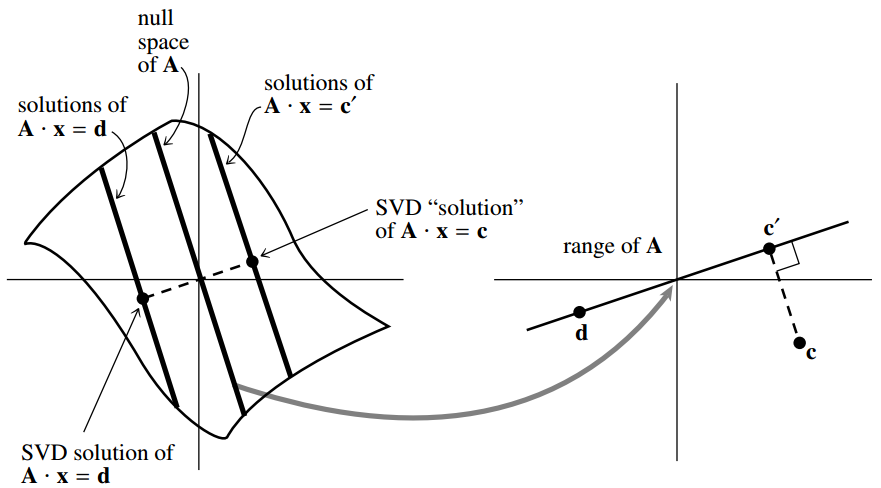
\includegraphics[scale=0.42]{svd.png}}
\end{figure}  


\end{frame}

%%%%%%%%%%%%%%%%%%%%%%%%%%%%%%%%%%%%%%%%%%%%

\begin{frame}{Motivation}

\frametitle{Motivation}
%\framesubtitle{continued}
\framesubtitle{The singular values of $A$}
%\section{Matrix decomposition}

For the curious mind, the \emph{singular} values of $A$ is as follows
\begin{equation*}
\begin{aligned}
\sigma_1 & = & 6\sqrt{10} \\
\sigma_2 & = & 3\sqrt{10} \\
\sigma_3 & = & 0
\end{aligned}.
\end{equation*}
They correspond to $||Av_i|| = \sigma_i $
\end{frame}

%%%%%%%%%%%%%%%%%%%%%%%%%%%%%%%%%%%%%%%%%%%%

\begin{frame}{Motivation}

\frametitle{Motivation}
%\framesubtitle{continued}
\framesubtitle{The singular values of $A$ cont.}
%\section{Matrix decomposition}
Explicitly for $\sigma_2$ we have
\begin{equation*}
A\mathbf{v}_2 = 
\begin{bmatrix}4 & 11 & 14 \\8 & 7 & -2 \end{bmatrix}
\begin{bmatrix}-2/3 \\ -1/3 \\ 2/3 \end{bmatrix} =
\begin{bmatrix}3 \\ -9 \end{bmatrix}
\end{equation*}
and then we take the norm
\begin{equation*}
\implies
 \sigma_i = ||Av_i|| = 3\sqrt{10}
\end{equation*}


\end{frame}

%%%%%%%%%%%%%%%%%%%%%%%%%%%%%%%%%%%%%%%%%%%%

\begin{frame}{Motivation}

\frametitle{Motivation}
%\framesubtitle{continued}
\framesubtitle{Geometric interpretation of singular values}
%\section{Matrix decomposition}

The two first singular values of $A$ corresponds to the length of the semiaxis of an ellipse

\begin{figure}[h] \centering{
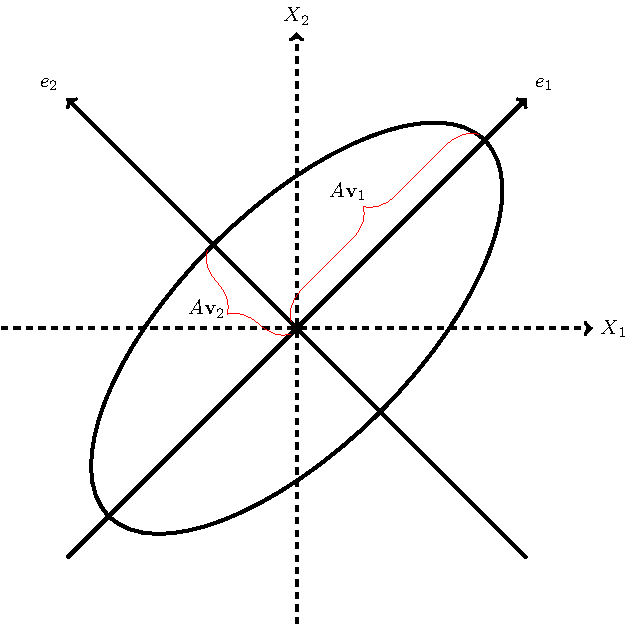
\includegraphics[scale=0.50]{ellipse.pdf}}
\end{figure}  

\end{frame}

%%%%%%%%%%%%%%%%%%%%%%%%%%%%%%%%%%%%%%%%%%%%
\section{Theory}

\begin{frame}{Definition}

\frametitle{Definition}
%\framesubtitle{continued}
\framesubtitle{Singular Value Decomposition}
%\section{Matrix decomposition}
The decomposition of $A$ involves an $m \times n$ matrix $\Sigma$ of the form
\begin{equation}
\Sigma = \begin{bmatrix}D & 0 \\ 0 & 0 \end{bmatrix}.
\end{equation}
where $D$ is an $r \times r$ diagonal matrix (r is the rank of $A$)
\end{frame}

%%%%%%%%%%%%%%%%%%%%%%%%%%%%%%%%%%%%%%%%%%%%

\begin{frame}{Theorem}

\frametitle{Theorem}
%\framesubtitle{continued}
\framesubtitle{Singular Value Decomposition}
%\section{Matrix decomposition}
$U$ is $m\times n$, $\Sigma$ is $n\times n$ and
$V$ is $n\times n$,
\begin{equation}
A = U\Sigma V^*
\end{equation}
where $U$, $V$ are orthogonal and its positive diagonal
entries is called the \emph{SVD} of $A$.

\end{frame}

%%%%%%%%%%%%%%%%%%%%%%%%%%%%%%%%%%%%%%%%%%%%

\begin{frame}{Proof}

\frametitle{Proof}
\framesubtitle{Singular Value Decomposition}
\textit{catch me in the break if you are interested}
\\
... since $V$ is orthogonal matrix, $U\Sigma V^* = AUV^T = A$

\end{frame}

%%%%%%%%%%%%%%%%%%%%%%%%%%%%%%%%%%%%%%%%%%%%
\section{The project}
\begin{frame}{The Project}

\frametitle{The Project}
\framesubtitle{Singular Value Decomposition}

Implement this in Python given constraints and a set of tasks.

\end{frame}

%%%%%%%%%%%%%%%%%%%%%%%%%%%%%%%%%%%%%%%%%%%%

\begin{frame}{The Project}

\frametitle{The Project}
\framesubtitle{Singular Value Decomposition}

In theory we can follow the following steps
\begin{enumerate}
\item Find the orthogonal diagonalization of $A^T A$
\item Set up $V$ and $\Sigma$
\item Construct $U$
\item Check singular values against eigenvalues ($||Av_i|| = \sigma_i $)
\end{enumerate}

\end{frame}

%%%%%%%%%%%%%%%%%%%%%%%%%%%%%%%%%%%%%%%%%%%%

\begin{frame}{The Project}

\frametitle{Reality check}
\framesubtitle{Singular Value Decomposition}

\textbf{But numerical linear algebra is reality}\\...which means \emph{IEEE-754} and
64-bit FPUs.

\end{frame}

%%%%%%%%%%%%%%%%%%%%%%%%%%%%%%%%%%%%%%%%%%%%

\begin{frame}{The Project}

\frametitle{Reality check}
\framesubtitle{Singular Value Decomposition}

SVD is considered a robust and numerically stable method, but a \emph{rank deficient\footnote{we have to guess more or less}} matrix will not produce exact zeroes for singular values. This is mainly due to finite numerical precision (IEEE-754 etc).

\end{frame}

%%%%%%%%%%%%%%%%%%%%%%%%%%%%%%%%%%%%%%%%%%%%

\begin{frame}{The Project}

\frametitle{The Project}
\framesubtitle{Requirements}

Requirements for the project
\begin{enumerate}
\item Givens rotations (to bring back $c$ to the x-axis)
\item Use Python
\item Visualize the computation (decomposition)
\item Have fun
\end{enumerate}

\end{frame}

%%%%%%%%%%%%%%%%%%%%%%%%%%%%%%%%%%%%%%%%%%%%

\begin{frame}{The Project}

\frametitle{The Project}
\framesubtitle{Implementation}

\textbf{How it was done}
\begin{enumerate}
\item Paper and pen and a good reference\footnote{Numerical Recipes In C, etc.}
\item A few keystrokes, i.e. Python is a reduced \emph{Lisp}
\item Emacs, git and Latex
\item MATLAB (as a reference)
\end{enumerate}


\end{frame}

%%%%%%%%%%%%%%%%%%%%%%%%%%%%%%%%%%%%%%%%%%%%

\begin{frame}{The Project}

\frametitle{The Project}
\framesubtitle{Challenges}

Well, \textbf{software development} and \textbf{numerical analysis}
\begin{itemize}
\item will test your skills (to some extent at least)
\item will learn you something new
\end{itemize}

\end{frame}

%%%%%%%%%%%%%%%%%%%%%%%%%%%%%%%%%%%%%%%%%%%%

\begin{frame}{The Project}

\frametitle{The Project}
\framesubtitle{Challenges}

\textbf{Now, \emph{just} one thing remains...}\\


\end{frame}

%%%%%%%%%%%%%%%%%%%%%%%%%%%%%%%%%%%%%%%%%%%%

\begin{frame}{The Project}

\frametitle{The Project}
\framesubtitle{Challenges}

Go home and decompose some matrices!

\end{frame}

%%%%%%%%%%%%%%%%%%%%%%%%%%%%%%%%%%%%%%%%%%%%

\begin{frame}{The Project}

\frametitle{The Project}
\framesubtitle{Checkout the source}

Checkout the project\footnote{there will be updates}
\begin{center}
\texttt{http://github.com/joastbg/python-svd}
\end{center}

\end{frame}

%%%%%%%%%%%%%%%%%%%%%%%%%%%%%%%%%%%%%%%%%%%%

\begin{frame}{The Project}

\frametitle{The Project}
\framesubtitle{Thanks and have a nice summer}

\begin{center}
\textbf{Thanks!}
\end{center}

\end{frame}

%%%%%%%%%%%%%%%%%%%%%%%%%%%%%%%%%%%%%%%%%%%%


\end{document}



